\documentclass[../_main/handlingar.tex]{subfiles}

\begin{document}
\motionssvar
Till skillnad från tidigare års phøs odlar alla manliga medlemmar i årets upplaga skägg. Styrelsen tycker dessutom att motionen är ytterst oseriös då motionären lagt fram ett förslag på perukset som utgått ur partykungens sortiment, se bild. Motionären vet inte heller att utskottet består av totalt sex stycken phøs.

\begin{center}
	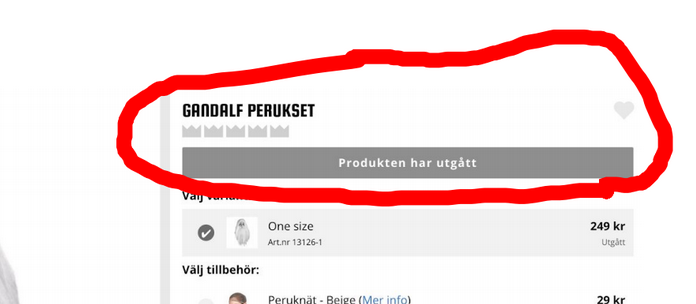
\includegraphics[width=12cm,height=6cm]{skagg2.PNG}
\end{center}

\newpage
I E-sektionens reglemente, \S10:2:L står det även följande:

\subsubsection{10:2:L Funktionärerna i Nolleutskottet, NollU}

\begin{emptylist}
    \item Øverphøsare (u)
        \begin{dashlist}
            \item Har det övergripande ansvaret för nollningen.
            \item Ansvarar för nollningsaktiviteter och nolleuppdrag.
            \item Ansvarar för rekryteringen av Co-phøs och Øvergudsphaddrar.
            \item Deltar aktivt i TLTH:s gemensamma planering inför nollningen.
        \end{dashlist}
    \item Co-phøsare (5)
        \begin{dashlist}
          \item Bistår Øverphøset i dennes arbete.
          \item Ett Co-phøs ansvarar för den ekonomiska redovisningen av nollningen.
          \item Ett Co-phøs ansvarar för rekryteringen av phaddrarna.
          \item Väljs av styrelsen på rekommendation av Øverphøset och avgående valberedning.
        \end{dashlist}
    \item Övergudphadder (2)
        \begin{dashlist}
          \item Ansvarar tillsammans med ett Co-phøs för phadderverksamheten.
          \item Väljs av styrelsen på rekommendation av Øverphøset, Co-phøsen och avgående
          valberedning.
        \end{dashlist}
\end{emptylist}
Som synes står ingenting om skäggväxt.

Därför yrkar styrelsen på 
\begin{attsatser}
    \att avslå motionen i sin helhet
\end{attsatser}

\begin{signatures}{1}
    \ist
    \signature{Daniel Bakic}{Ordförande}
\end{signatures}

\end{document}
